\documentclass[compsoc,conference,letterpaper,fleqn]{IEEEtran}
 
\usepackage{cite}
\usepackage{amsmath,amsfonts,amssymb,amsthm}
\usepackage{thmtools}
\usepackage{stmaryrd}
\usepackage{natbib}
\usepackage{url}
\usepackage{array}
\usepackage{arydshln}
\usepackage{ifthen}
\usepackage{ifpdf}
\usepackage{verbatim}
\usepackage{mathpartir}
\usepackage{listings}
\usepackage{hyperref}
\usepackage{natbib}
\lstset{
  basicstyle=\ttfamily,
  columns=fullflexible,
  keepspaces=true,
  mathescape
}

\usepackage{rotating}

\usepackage{afterpage}

\usepackage{mathtools}
\DeclarePairedDelimiter\ceil{\lceil}{\rceil}
\DeclarePairedDelimiter\floor{\lfloor}{\rfloor}

\usepackage{enumitem}
\newlist{enumproof}{enumerate}{10}
\setlist[enumproof]{label*=\arabic*.}

\usepackage{tikz}
\usepackage{multirow,bigdelim}

% %make latex preview-mode work with natbib...
% \usepackage[displaymath,floats,graphics,textmath,footnotes]{preview}

\newtheorem{theorem}{Theorem}

\newcommand{\forcenewline}{$\phantom{v}$\\}
\newcommand{\judgment}[2]{\paragraph{#1}\hspace{\stretch{1}}\fbox{$#2$}}

\newcommand{\update}[2]{[#1 \mapsto #2]}
\newcommand{\sem}[1]{\left\llbracket #1 \right\rrbracket}

% Math notation
\newcommand{\restrictfun}[1]{|_{#1}}
\newcommand{\parfun}{\rightharpoonup}
\newcommand{\finparfun}{\xrightharpoonup{\textit{\tiny{fin}}}}
\newcommand{\monnefun}{\xrightarrow{\textit{\tiny{mon, ne}}}}
\newcommand{\monfun}{\xrightarrow{\textit{\tiny{mon}}}}
\newcommand{\nefun}{\xrightarrow{\textit{\tiny{ne}}}}
\newcommand{\fun}{\rightarrow}
\newcommand{\defeq}{\stackrel{\textit{\tiny{def}}}{=}}
\newcommand{\nequal}[1][n]{\stackrel{\tiny{#1}}{=}}
\renewcommand{\nsim}[1][n]{\stackrel{\tiny{#1}}{\simeq}}

\newcommand\subsetsim{\mathrel{\ooalign{\raise.2ex\hbox{$\subset$}\cr
      \hidewidth\lower.8ex\hbox{\scalebox{0.9}{$\sim$}}\hidewidth\cr}}}
\newcommand\supsetsim{\mathrel{\ooalign{\raise.2ex\hbox{$\supset$}\cr
      \hidewidth\lower.8ex\hbox{\scalebox{0.9}{$\sim$}}\hidewidth\cr}}}
\newcommand{\nsubsim}[1][n]{\stackrel{\tiny{#1}}{\subsetsim}}
\newcommand{\nsupsim}[1][n]{\stackrel{\tiny{#1}}{\supsetsim}}

\newcommand{\nsubeq}[1][n]{\stackrel{\tiny{#1}}{\subseteq}}
\newcommand{\nsupeq}[1][n]{\stackrel{\tiny{#1}}{\supseteq}}

\newcommand{\union}{\mathbin{\cup}}
\DeclareMathOperator{\dom}{dom}
\newcommand{\blater}{\mathop{\blacktriangleright}}
\newcommand{\id}{\var{id}}
\newcommand{\undefined}{\mathit{undefined}}

\newcommand{\powerset}[1]{\mathcal{P}(#1)}

\newcommand{\false}{\mathit{false}}
\newcommand{\true}{\mathit{true}}


% cofes
\newcommand{\cofe}{c.o.f.e.}
\newcommand{\cofes}{\cofe{}'s}
\newcommand{\CatC}{\mathbb{C}}
\newcommand{\CatP}{\mathbb{P}}

% Comments
\newcommand\lau[1]{{\color{purple} \sf \footnotesize {LS: #1}}\\}
\newcommand\dominique[1]{{\color{purple} \sf \footnotesize {DD: #1}}\\}
\newcommand\lars[1]{{\color{purple} \sf \footnotesize {LB: #1}}\\}

% Variables
\newcommand{\var}[1]{\mathit{#1}}
\newcommand{\hs}{\var{ms}}
\newcommand{\ms}{\hs}
\newcommand{\hv}{\var{hv}}
\newcommand{\rv}{\var{rv}}
\newcommand{\lv}{\var{lv}}
\newcommand{\gl}{\var{g}}
\newcommand{\pc}{\mathit{pc}}
\newcommand{\pcreg}{\mathrm{pc}}
\newcommand{\addr}{\var{a}}
\newcommand{\offset}{\var{offset}}
\newcommand{\word}{\var{w}}
\newcommand{\start}{\var{base}}
\newcommand{\addrend}{\var{end}}
\newcommand{\pwlv}{\var{pwl}}
\newcommand{\mem}{\var{mem}}
\newcommand{\reg}{\var{reg}}
\newcommand{\heapseg}{\var{ms}}
\newcommand{\heap}{\var{mem}}
\newcommand{\mode}{\var{mode}}
\newcommand{\perm}{\var{perm}}
\newcommand{\permp}{\var{permPair}}
\newcommand{\roll}{\var{roll}}
\newcommand{\instr}{\var{instr}}
\newcommand{\stdcap}[1][(\perm,\gl)]{\left(#1,\start,\addrend,\addr \right)}
\newcommand{\adv}{\var{adv}}
\newcommand{\msframe}{ms_\var{frame}}
\newcommand{\link}{\var{link}}
\newcommand{\stk}{\var{stk}}
\newcommand{\flag}{\var{flag}}
\newcommand{\nwl}{\var{nwl}}
\newcommand{\pwl}{\var{pwl}}
\newcommand{\sta}{\var{sta}}
\newcommand{\cnst}{\var{cnst}}
\newcommand{\olf}{\var{offsetLinkFlag}}
\newcommand{\prp}{\var{prp}}
\newcommand{\env}{\var{env}}
\newcommand{\cls}{\var{cls}}
\newcommand{\unused}{\var{unused}}
\newcommand{\act}{\var{act}}


% Memory projections
\newcommand{\plainproj}[1]{\mathrm{#1}}
\newcommand{\memheap}[1][\Phi]{#1.\plainproj{mem}}
\newcommand{\memreg}[1][\Phi]{#1.\plainproj{reg}}

\newcommand{\updateHeap}[3][\Phi]{#1\update{\plainproj{mem}.#2}{#3}}
\newcommand{\updateReg}[3][\Phi]{#1\update{\plainproj{reg}.#2}{#3}}

% Configuration end states
\newcommand{\failed}{\mathit{failed}}
\newcommand{\halted}{\mathit{halted}}

% Functions
\newcommand{\plainfun}[2]{
  \ifthenelse{\equal{#2}{}}
  {\mathit{#1}}
  {\mathit{#1}(#2)}
}
\newcommand{\decode}{\plainfun{decode}{}}
\newcommand{\encode}{\plainfun{encode}{}}
\newcommand{\encodePerm}{\mathit{encodePerm}}
\newcommand{\encodePermPair}{\plainfun{encodePermPair}{}}
\newcommand{\encodeLoc}{\mathit{encodeLoc}{}}
\newcommand{\decodePermPair}{\plainfun{decodePermPair}}
\newcommand{\decodePerm}[1]{\plainfun{decodePerm}{#1}}
\newcommand{\updatePcPerm}[1]{\plainfun{updatePcPerm}{#1}}

\newcommand{\executeAllowed}[1]{\plainfun{executeAllowed}{#1}}
\newcommand{\nonZero}[1]{\plainfun{nonZero}{#1}}
\newcommand{\readAllowed}[1]{\plainfun{readAllowed}{#1}}
\newcommand{\writeAllowed}[1]{\plainfun{writeAllowed}{#1}}
\newcommand{\withinBounds}[1]{\plainfun{withinBounds}{#1}}
\newcommand{\stdUpdatePc}[1]{\plainfun{updatePc}{#1}}

\newcommand{\readCond}[1]{\plainfun{readCondition}{#1}}
\newcommand{\writeCond}[1]{\plainfun{writeCondition}{#1}}
\newcommand{\execCond}[1]{\plainfun{executeCondition}{#1}}
\newcommand{\entryCond}[1]{\plainfun{enterCondition}{#1}}

\newcommand{\revokeTemp}[1]{\plainfun{revokeTemp}{#1}}
\newcommand{\erase}[2]{\floor*{#1}_{\{#2\}}}
\newcommand{\activeReg}[1]{\plainfun{active}{#1}}

% World operations
\newcommand{\future}{\mathbin{\sqsupseteq}}
\newcommand{\pub}{\var{pub}}
\newcommand{\priv}{\var{priv}}
\newcommand{\futurewk}{\mathbin{\sqsupseteq}^{\var{pub}}}
\newcommand{\futurestr}{\mathbin{\sqsupseteq}^{\var{priv}}}
\newcommand{\heapSat}[3][\heap]{#1 :_{#2} #3}
\newcommand{\memSat}[3][n]{\heapSat[#2]{#1}{#3}}
\newcommand{\memSatPar}[4][n]{\heapSat[#2]{#1 , #4}{#3}}

\newcommand{\monwknefun}{\xrightarrow[\text{\tiny{$\futurewk$}}]{\textit{\tiny{mon, ne}}}}
\newcommand{\monstrnefun}{\xrightarrow[\text{\tiny{$\futurestr$}}]{\textit{\tiny{mon, ne}}}}


% Assembly labels
\newcommand{\codelabel}[1]{\mathit{#1}}
\newcommand{\init}{\codelabel{init}}
\newcommand{\malloc}{\codelabel{malloc}}
\newcommand{\counter}{\codelabel{counter}}
\newcommand{\iocap}{\codelabel{iocap}}

% Type(s)
\newcommand{\type}[1]{\mathrm{#1}}
\newcommand{\asmType}{\plaindom{AsmType}}


% Domains
\newcommand{\plaindom}[1]{\mathrm{#1}}
\newcommand{\Caps}{\plaindom{Cap}}
\newcommand{\Words}{\plaindom{Word}}
\newcommand{\Addrs}{\plaindom{Addr}}
\newcommand{\ExecConfs}{\plaindom{ExecConf}}
\newcommand{\RegName}{\plaindom{RegisterName}}
\newcommand{\Regs}{\plaindom{Reg}}
\newcommand{\Heaps}{\plaindom{Mem}}
\newcommand{\Mems}{\Heaps}
%\newcommand{\HeapSegments}{\plaindom{MemSegment}}
\newcommand{\HeapSegments}{\plaindom{MemSeg}}
\newcommand{\MemSegments}{\HeapSegments}
\newcommand{\Confs}{\plaindom{Conf}}
\newcommand{\Instrs}{\plaindom{Instructions}}
\newcommand{\nats}{\mathbb{N}}
\newcommand{\ints}{\mathbb{Z}}
\newcommand{\Perms}{\plaindom{Perm}}
\newcommand{\Globals}{\plaindom{Global}}

\newcommand{\Rel}{\plaindom{Rel}}
\newcommand{\Rels}{\plaindom{Rels}}
\newcommand{\States}{\plaindom{State}}
\newcommand{\RegionNames}{\plaindom{RegionName}}
\newcommand{\Regions}{\plaindom{Region}}
\newcommand{\Reg}{\plaindom{Reg}}
\newcommand{\Worlds}{\plaindom{World}}
\newcommand{\Wor}{\plaindom{Wor}}
\newcommand{\Worwk}{\Wor_{\futurewk}}
\newcommand{\Worstr}{\Wor_{\futurestr}}
\newcommand{\xiwk}{\xi_{\var{wk}}}
\newcommand{\xistr}{\xi_{\var{str}}}
\newcommand{\StorePred}{\plaindom{MemSegPred}}
\newcommand{\UPred}[1]{\plaindom{UPred}(#1)}
\newcommand{\DCPred}[1]{\plaindom{P}^\downarrow(#1)}

\newcommand{\Views}{\plaindom{View}}

% LR
\newcommand{\intr}[2]{\mathcal{#1}}
\newcommand{\valueintr}[1]{\intr{V}{#1}}
\newcommand{\exprintr}[1]{\intr{E}{#1}}
\newcommand{\contintr}[1]{\intr{K}{#1}}
\newcommand{\regintr}[1]{\intr{R}{#1}}
\newcommand{\stdvr}{\valueintr{\asmType}}
\newcommand{\stder}{\exprintr{\asmType}}
\newcommand{\stdrr}{\regintr{\asmType}}
\newcommand{\stdkr}{\contintr{\asmType}}
\newcommand{\observations}{\mathcal{O}}
\newcommand{\npair}[2][n]{\left(#1,#2 \right)}

% Reference register/memory
\newcommand{\refreg}[1]{\lfloor #1 \rfloor}
\newcommand{\refheap}[1]{\langle #1 \rangle_m}

% Instructions
% No arguments
\newcommand{\zinstr}[1]{\mathtt{#1}}
\newcommand{\fail}{\zinstr{fail}}
\newcommand{\halt}{\zinstr{halt}}
% One argument
\newcommand{\oneinstr}[2]{\zinstr{#1} \; #2}
\newcommand{\jmp}[1]{\oneinstr{jmp}{#1}}
% Two arguments
\newcommand{\twoinstr}[3]{\zinstr{#1} \; #2 \; #3}
\newcommand{\restricttwo}[2]{\twoinstr{restrict}{#1}{#2}}
\newcommand{\jnz}[2]{\twoinstr{jnz}{#1}{#2}}
\newcommand{\isptr}[2]{\twoinstr{isptr}{#1}{#2}}
\newcommand{\geta}[2]{\twoinstr{geta}{#1}{#2}}
\newcommand{\getb}[2]{\twoinstr{getb}{#1}{#2}}
\newcommand{\gete}[2]{\twoinstr{gete}{#1}{#2}}
\newcommand{\getp}[2]{\twoinstr{getp}{#1}{#2}}
\newcommand{\getl}[2]{\twoinstr{getl}{#1}{#2}}
\newcommand{\move}[2]{\twoinstr{move}{#1}{#2}}
\newcommand{\store}[2]{\twoinstr{store}{#1}{#2}}
\newcommand{\load}[2]{\twoinstr{load}{#1}{#2}}
\newcommand{\lea}[2]{\twoinstr{lea}{#1}{#2}}
% Three arguments
\newcommand{\threeinstr}[4]{\zinstr{#1} \; #2 \; #3 \; #4}
\newcommand{\restrict}[3]{\threeinstr{restrict}{#1}{#2}{#3}}
\newcommand{\subseg}[3]{\threeinstr{subseg}{#1}{#2}{#3}}
\newcommand{\plus}[3]{\threeinstr{plus}{#1}{#2}{#3}}

% Permissions
\newcommand{\plainperm}[1]{\mathrm{#1}}
\newcommand{\noperm}{\plainperm{o}}
\newcommand{\readonly}{\plainperm{ro}}
\newcommand{\readwrite}{\plainperm{rw}}
\newcommand{\exec}{\plainperm{rx}}
\newcommand{\entry}{\plainperm{e}}
\newcommand{\rwx}{\plainperm{rwx}}
% PWL permissions
\newcommand{\readwritel}{\plainperm{rwl}}
\newcommand{\rwl}{\readwritel}
\newcommand{\rwlx}{\plainperm{rwlx}}

% Global/local
\newcommand{\local}{\plainperm{local}}
\newcommand{\glob}{\plainperm{global}}

\newcommand{\localityReg}{\var{localityReg}}
\newcommand{\localReg}{\var{localReg}}
\newcommand{\globalReg}{\var{globalReg}}

% Views
\newcommand{\plainview}[1]{\mathrm{#1}}
\newcommand{\perma}{\plainview{perm}}
\newcommand{\temp}{\plainview{temp}}
\newcommand{\revoked}{\plainview{revoked}}

% OP sem
\newcommand{\diverge}[1][n]{\not\Downarrow_{#1}}
\newcommand{\step}[1][]{\rightarrow_{#1}}

% Conv defs
\newcommand{\lookingat}[3]{\ensuremath{#1} \text{ is looking at } \ensuremath{#2} \text{ followed by } \ensuremath{#3}}
\newcommand{\pointstostack}[3]{\ensuremath{#1} \text{ points to stack with } \ensuremath{#2} \text{ used and } \ensuremath{#3} \text{ unused}}
\newcommand{\nonlocal}[1]{\ensuremath{#1} \text{ is non-local}}

% Macros
\newcommand{\scall}[3]{\mathtt{scall} \; #1([#2],[#3])}





\usepackage[colorinlistoftodos,prependcaption,textsize=tiny]{todonotes}


% domi: IEEEtran.cls sets font size to 10bp, apparently.
% not sure what the difference is with 10pt.
\DeclareMathSizes{10bp}{8}{7}{6}

%\def\IEEEbibitemsep{0pt}

\makeatletter
\setlength\mpr@andskip{1em}
\def\mpr@lineskip{5em}
\def\MathparLineskip{\mpr@lesslineskip}
\makeatother

\newlength{\oldmathindent}
\newenvironment{withmathindent}[1]{\setlength{\oldmathindent}{\mathindent}\setlength{\mathindent}{#1}}{\setlength{\mathindent}{\oldmathindent}}



\begin{document}
\setlength{\mathindent}{.2cm}

\title{Reasoning about a Capability Machine with Local Capabilities\\
 Provably Safe Stack and Return Pointer Management (without OS Support).}


\author{%
\IEEEauthorblockN{Lau~Skorstengaard}
\IEEEauthorblockA{Aarhus University, Denmark\\
Email: lau@cs.au.dk} \and
\IEEEauthorblockN{Dominique~Devriese}
  \IEEEauthorblockA{iMinds-DistriNet, KU Leuven, Belgium\\
Email: dominique.devriese@cs.kuleuven.be} \and
\IEEEauthorblockN{Lars~Birkedal}\IEEEauthorblockA{Aarhus University, Denmark\\
Email: birkedal@cs.au.dk}}

\maketitle

\begin{abstract}
  abc
\end{abstract}

\section*{Terminology ?}

\emph{capability safe}: 
Our unary logical relation is a semantic \emph{definition}
of which values for the
pc / register-file / word are capability safe. 

\emph{adversary}: It doesn't sound ``sexy'' to constantly say ``an untrusted
piece of code'' should we adopt the convention that adversary refers
to an unstrusted piece of code?

\emph{memory}  we don't make a distinction between memory and memory
segments in the text  (to do so properly, we would need to explain why
assumptions
are reasonable, given that a real machine has finite memory, but we
need infinite domain for malloc spec, etc.)


\section{Introduction}
\label{sec:introduction}
\todo[inline]{See the latex comments for the next paragraphs!}

Compromising software security is often based on attacks that break programming
language properties relied upon by software authors, such as control flow
integrity, local state encapsulation etc. Commodity processors offer little
support for defending against such attacks: they offer security primitives with
only coarse-grained memory protection and limited compartmentalization
scalability. As a result, defenses against attacks on control flow integrity and
local state encapsulation are either limited to only certain common forms of
attacks (leading to an attack-defense arms race) or rely on techniques like
machine code rewriting
(e.g.~\cite{wahbe_efficient_1993,abadi_control-flow_2005}), machine code
verification (e.g.~\cite{morrisett_system_1999}), virtual machines with a native
stack (e.g.~the JVM~\cite{lindholm_java_2014}) or
randomization~\cite{forrest_building_1997}. The latter techniques essentially
emulate protection techniques on existing hardware, at the cost of performance,
system complexity and/or security.

\emph{Capability machines} are a type of processors, intended to remediate these
limitations by presenting a better security model at the hardware level. They
are based on old ideas
(e.g.~\cite{Carter:1994:HSF:195473.195579,Dennis:1966:PSM:365230.365252,shapiro_eros:_1999}),
but have recently received renewd interest with particularly the CHERI project
proposing new ideas and tackling practical challenges like backwards
compatibility and realistic OS
support~\cite{Watson2015Cheri,Woodruff:2014:CCM:2665671.2665740}. Capability
machines tag every word (in the register file and in memory) to enforce a
strict separation between numbers and capabilities, a kind of pointers carrying
some kind of authority. Memory capabilities carry the authority to read and/or
write to a range of memory locations. Additionally, the details vary but all
capability machines offer some form of \emph{object capabilities}, which
represent the authority to invoke a piece of code without exposing the code's
encapsulated private state (e.g. the M-Machine's enter capabilities or CHERI's
sealed code/data pairs).

Unlike for commodity processors, the security primitives on capability machines
lend themselves well to the enforcement of properties like local state
encapsulation and control-flow integrity. Potentially, they will enable new
compilation schemes that enforce such properties in a way that is efficient but
also 100\% watertight (ideally evidenced by a mathematical proof, guaranteeing
that we do not end up in a new attack-defense arms race). However, there is
still a lot that needs to happen to attain this goal. For example, it is quite
non-trivial to devise a compilation scheme adapted to the details of a specific
language's notion of encapsulation (e.g. encapsulation of private member
variables in OO languages often behaves quite differently than encapsulation of
private state in ML-like languages). And even if such a scheme were defined, a
formal proof depends on a formalisation of the encapsulation provided by the
capability machine at hand.

A similar problem is the enforcement of control-flow integrity on capability
machines. An interesting approach is taken in CheriBSD. They drop the standard
contiguous C stack and split it into a central, trusted shadow stack, managed by
trusted call and return instructions\footnote{These call and return instructions
  are implemented by CheriBSD and special support from the CHERI processor makes
  them very fast to invoke.}, and disjoint, per-component
stacks~\citep{Watson2015Cheri}. For preventing illegal use of stack references,
the approach relies on \emph{local capabilities}, a type of capabilities offered
by CHERI that can be passed over a function invocation \emph{temporarily}, for
the duration of the invocation, and revoked afterwards. However, a lot of
details remain to be filled in (e.g. how to combine a trusted shadow stack with
(potentially) cross-domain function pointers in a scalable way?) and there is no
argument that this enforcement of CFI is watertight.

In this paper, we make progress towards the goal of efficient, provably
watertight enforcement of encapsulation and control-flow integrity on capability
machines.  Specifically, we make the following contributions:
\begin{itemize}
\item We formalise a simple but representative capability machine featuring
  local capabilities much like CHERI's, and define its operational semantics.
\item We define a novel stack management discipline for enforcing control-flow
  integrity and encapsulation of local state on the stack. The discipline relies
  solely on local capabilities (used to represent stack and return pointers) and
  does not require OS support in the form of a trusted shadow stack or special
  call and return instructions. It also does not require separate per-component
  stacks and instead works with a single, fairly standard contiguous stack. It
  supports higher-order cross-component calls (e.g. (potentially)
  cross-component function pointers) and can be efficient assuming one
  additional piece of processor support: an instruction for efficiently clearing
  a range of memory.
\item We provide a theorem (capability-safety) that is (by far) the most general
  and powerful formulation of the guarantees offered by a capability machine.
  The theorem also expresses the specific guarantees offered by the machine for
  local capabilities. It is very general and not tied to a specific ABI or a
  specific way of using the system's capabilities.
\item The above theorem is formulated in terms of a unary step-indexed logical
  relation with recursively defined Kripke worlds. It is inspired by one used by
  \cite{Devriese:2016ObjCap} for capability-safety in a JavaScript-like lambda
  calculus, but has two novel technical characteristics. The natural CPS style
  of assembly code with return pointers as continuations is modeled using a
  \emph{single} orthogonal closure, rather than the biorthogonal closure that
  has been previously used for lambda calculi. Perhaps more surprisingly, we
  show that the special nature of local capabilities can be elegantly expressed
  using a variant of an idea that has been used by
  \cite{Dreyer:2010:IHS:1863543.1863566} to express well-bracketedness
  guarantees in a lambda calculus: Kripke worlds with a weak and a strong future
  world relations. Interestingly, the two future world relations generally work
  very similarly to Dreyer et al.'s, except that they turn up in quite a
  different place in the logical relation.
\item We demonstrate the power of our results by applying them to challenging
  examples, specifically constructed to demonstrate local state encapsulation
  and control-flow integrity guarantees in the presence of cross-component
  function pointers. The examples demonstrate both the power of our formulation
  of capability-safety and our stack management discipline.
\end{itemize}

% % Possible high-level intros:
% % 0) Arms race compilers
% %
% % 1) Security guarantees vs obstacles / arms race
% \begin{comment}
%   Security on processors is today subject to an arms race between
%   processor manufacturers and hackers. On the hacker side, a constant
%   effort is put into exploiting current processor designs and
%   circumventing the security measures set in place to prevent known
%   exploits. On the processor manufacturer side, new security measures
%   are put in place to prevent new exploits. The arms race would come
%   to a grinding halt if the security meassures provided more than
%   obstacles and actually provided low-level security guarantees. One
%   kind of low-level machines that provide low-level security is a
%   capability machine.
% \end{comment}
% % 2) Fully abstract compilation
% High-level languages provide guarantees such as encapsulation of local
% state and well-bracketedness of function calls. These guarantees are
% often relied upon when reasoning about the correctness and security of
% a program. High-level programs are compiled to machine code, so in
% order to rely on the correctness and security guarantees provided by
% the high-level language, it needs to be proven that the translation
% preserves these properties. Translated programs often interact with
% machine code that is not translated from the same high-level language,
% so in order to preserve the guarantees from the high-level languages,
% the low-level machine needs to provide some kind of security
% guarantees. In other words, a target of secure compilation needs to
% provide some security guarantees. Modern processors provide many
% security meassures, but very little in terms of guarantees. A machine
% that provides some means of security guarantees is a capability machine.

% % 3) Memory access-control
% % I don't like this angle and can't find a good way to sell it.

% % 4) History
% % Proposals throughout history.
% % Lack of formal account of properties-guarantees.

% %%% a)
% % Current low-level protection coarse grained memory protection or
% % properties of high-level languages are not really enforced?

% % Capability machines offer fine-grained memory protection
% % Too technical
% A capability machine is a low-level machine that offers fine-grained
% memory protection.
% % Capability machines and unforgeable tokens for memory access. 
% This is done by introducing unforgeable tokens to
% the machine. These tokens are called capabillities and grant a kind of
% authority and a range of authority. 
% % Dynamic checks encapsulation, formal model

%  We will refer to the capabilities
% that grant a combination of read, write, or execute permission as memory
% capabilities. 
%  Capabilities with the necessary permissions must be
% presented every time an instruction that manipulates the memory is
% executed.

% Memory capabilities provide memory protection, but they do not provide
% a way to set up security domains. When you jump to an untrusted piece
% of code that is supposed to jump back to you, then you have to either
% revoke all your capabilities or pass to the piece of code you do not
% trust. This short coming can be overcome by adding something like the
% enter capability from the M-Machine\todo{add reference}. The enter
% capability is an opaque capability which can only be used for a
% jump. When jumped to it grants read and execute permission which
% allows the code that is now executing to read capabilities stored in
% memory. 
% The CHERI processor's ccall achieves a similar property\todo{Add reference}.

% Capabilities are irrevocable, so when we pass a capability has to
% an untrusted program, then we have to assume that the program keeps it
% around indefenitely. This means that we cannot reuse the piece of
% memory that the capability governs essentially creating a memory
% leak. The CHERI processor has a special kind of capabilities called
% \emph{local capabilities}\todo{reference?}\ that introduces a simple
% kind of temporal information control which allows for a simple kind of
% capability revocation. This is achieved by adding a tag to every
% capability that marks it as either local or global. Local capabilities
% can only be written through a capability with a new permission called
% \emph{permit write local}.
% % More about local capabilities.

% With just memory capabilities, enter capabailities, and local
% capabilities, the capability machine is very powerful and can
% enforce properties that high-level languages promise. In most
% high-level languages, we expect local state to be private and
% encapsulated. The memory capabilities make sure that local state
% cannot be accessed without a capability to do so. With the enter
% capabaility, we can regain control of local state after passing
% control to an untrusted piece of code which gives us encapsulation
% when control is passed to an untrusted program.

% Many high-level languages guarantee that function function calls are
% well-bracketed. This can easily be achieved by having a trusted call
% stack. On a capability machine, it is possible to enforce well
% barcketedness without a trusted stack. When ensuring well-bracketed
% the two main challenges calls are 1) preventing storage of return
% pointers and 2) encapsulation of the local stack frame. If we don't
% have the first property, then an adversary can store the return
% capability in a call and jump to it in a later call. If the local
% stack frame is not properly encapsulated, then an adversary can break
% the well-bracketedness by jumping to a different calls return
% capability.

% In order to deal with the two challenges, we make sure that all return
% capabilities are local and that there are no global capabilities with
% permit write local permission. This makes sure that there is no way to
% save a return capability in persistent local state.\lau{this does not really make
% sense as the local stack frame can be seen as local state} It is,
% however, to limiting to not provide any means to store the return
% capabilities as a piece of code may need to store a return capability
% before jumping to an adversary. It is therefore needed to provide a
% local capability with permit write local permission which can be used
% as a stack. The stack should now be the only place one can store the
% return capability, but it should also be the only place one can store
% the stack capability. 

% Using local return capabilities and putting a stack abstraction on a
% local capability permit write local capability is a good start, but as
% it turns out, it is not wnough. An adversary could do the following 
% \begin{enumerate}
% \item In a first invocation, fill the stack frame with copies of the
%   current stack capability.
% \item In a later call, the adversary may be able to load the stack
%   capability from the previous call.
% \item If we have used a larger part of the stack than in the first
%   call, then the adversary has access to part of our local stack frame.
% \end{enumerate}

% The above attack shows that it is tricky to ensure
% well-bracketedness. It raises the question whether it is possible to
% do so it is completely watertight. The attack utilized the stack, so
% it is necessary to have a trusted stack or can we do without? In
% general it raises the question, how do we reason about capability
% machines and local capabilities, so we are sure that what ever calling
% scheme we come up with actually provably ensures well-bracketed calls.

% In the following paper, we present the following contributions
% \begin{enumerate}
% \item 
% \end{enumerate}
 

%%% b)




% Examples of capability machines?


% Enter capabilities

% Local capabilities

% High-level languages often provide guarantees such as encapsulation of private state and well-bracketedness of calls - often not clear how well this is enforced. Just enforced when interacting with other programs written in the same high-level language or is it also guaranteed when interacting with assembly programs.

% High-level programs compiled to assembly can ensure these properties.

% 

\subsection{Introduce capability machines}
\subsection{Enforcing properties on a capability machine}

Privacy of local state using memory capabilities.
Encapsulation of private state using enter pointers or CHERI's ccall.
(mention in passing secure compilation, full abstraction)

\subsection{Well-bracketed control flow and encapsulation of stack frames}

Hard to enforce using standard capabilities:
\begin{itemize}
\item Well-bracketed control flow can be broken if the adversary stores return pointers.
(alternative: trusted stack)
\item Encapsulation of local stack frames can be broken if the adversary stores stack pointers.
\end{itemize}

\subsection{Local capabilities}

\begin{itemize}
\item Introduced by CHERI for this purpose.
\item Explain how they can be used for passing return pointers and stack pointers.
\item But this is not watertight.
\item Example attack:
\begin{itemize}
\item In a first invocation, adversary fills the entire unused part of the stack with copies of the current stack pointer
\item In a second invocation, adversary can load the old stack pointer of the stack
\item He now has access to private state that was pushed on the stack in between.
\end{itemize}
\item So:
\begin{itemize}
\item Can we make it (provably) watertight?
\item Is the trusted stack necessary? Why not just pass return pointers locally?
\item General question: How to reason about capability machines and
local capabilities?
\end{itemize}
\end{itemize}

\subsection{Contributions}

\begin{itemize}
\item Formal model of a simple but representative capability machine with local capabilities
\item Detailed study of how to do safe stack and return pointer management in this setting, taking into account:
\begin{itemize}
\item untrusted adversary
\item higher-order code: callbacks passed to and received from the adversary
\item efficient stack management
\item no OS support
\end{itemize}
\item Logical relation for reasoning about code in this capability machine
\item Fundamental theorem that expresses the guarantees offered by a capability machine for untrusted code
\item Technical contributions: reuse existing ideas in a new way:
\begin{itemize}
\item replace biorthogonal closure by a single orthogonal closure
because assembly languages remove the distinction between the
continuation and the arguments
\end{itemize}
\end{itemize}
LB: I think we should have some discussion of the flexibility /
  strength of our LR.  The LR defines which computations we think of
  as well-behaved.   
 We should give simple / trivial examples of
  code not in the LR. But we may also want to emphasize that the LR is 
  not too restricting, e.g., it does not enforce a certain calling
  scheme (examplied by Example \verb!f1! which
  does not use the stack and the following examples which do use the
  stack). This ties in to the discussion of biorthogonality, see the
  following paragraphs. 

LB: we need to relate this carefully to Hur-Dreyer, who used
      biorthogonality even though they also worked with an assembly
      language. (If I recall correctly, they assumed some properties
      of the low level language, which is why the biortho was the
      right ting, but we need to check.)

LS: It is my impression that they were interested in the relation
between high-level and low-level programs. They are therefore in
particular interested in low-level programs compiled from high-level
programs which means that the continuation is always invoked in the 
same way. Our realisation was that anything we pass as an argument 
in a "call" can be used as a continuation, so the continuation 
relation was redundant. Even though we do try to give our programs
some structure using the macros, our logical relation is strong enough
to handle unstructured programs as well.
\begin{itemize}
\item STSs with public/private transitions for dealing with local capabilities: play the same role as before, but in different places of the LR.
\end{itemize}
\begin{itemize}
\item Demonstrate all of this on several examples:
\begin{itemize}
\item security examples
\item the most challenging examples from existing literature on reasoning about well-bracketed control flow in lambda calculi
\item some compartmentalisation result?
\item whatever else we do..
\end{itemize}
\end{itemize}

\subsection{Outline}

\section{A capability machine with local capabilities}

Formalisation

Explain our model of linking

\section{Stack and return pointer management using local capabilities}

\begin{itemize}
\item Issues to consider:
\begin{itemize}
\item no global store-local capabilities
\item clearing the stack
\item clearing (some) registers
\item constructing return pointers
\item constructing callbacks
\item invoking the adversary's callbacks
\end{itemize}
\item Reusable macro-instructions for stack and return pointer management
\begin{itemize}
\item taking care of the stuff above
\end{itemize}
\end{itemize}

LB: maybe we can present the examples informally before the logical relation and then return to them after the logical relation (to present the formal properties) ?

\section{Logical relation}
In order to be able to reason about programs running on the capability
machine and prove properties such as well-bracketedness and
encapsulation about them, we define a unary logical relation.

% Intuition
The logical relation is a semantic model of all the words on the
capability machine that are definitely safe to give to an
adversary. Whether a capability is safe to give to an adversary
depends heavily on the contents of the memory since instructions as well
as capabilities may reside in memory. Hence we index the logical
relation over worlds, which are used to model the memory, and our logical
relation is thus an example of what is often referred to as a Kripke
logical relation. A world consists of a finite set of regions, and each region
can be understood as a protocol describing the possible evolution of
part of the memory. Memory changes during an
execution since new memory can be allocated and part of the existing
memory can change. We use two future world relations to capture
such changes to the memory in our model.
%

\subsection{Worlds}
\todo[inline]{Find a good place to describe monotonicity of
  interpretation function.}
\begin{figure}[htbp]
  \centering
  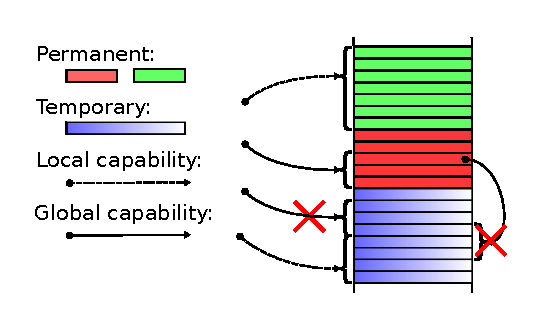
\includegraphics{w11}
  \caption{Relation between local and global capabilities and temporary and permanent regions.}
  \label{fig:cap-world}
\end{figure}
A world is a finite map from region names, modeled as natural numbers, to regions.
We have three types of regions: \emph{permanent}, \emph{temporary}, and \emph{revoked}.
%$\perma$, $\temp$, and $\revoked$. The
%$\perma$ and $\temp$ 
Each permanent and temporary region contains a state transition system, with
public and private transitions, which describes the protocol governing
the evolution of the memory described by the region, similarly to what
has been used in logical relations for high-level
languages~\cite{Ahmed:popl09,Dreyer:jfp12,Devriese:2016ObjCap}. 
The protocols imposed on memory by permanent regions stay in place
indefinitely. This means that any capability, local or global, can
depend on these protocols. The protocols imposed on memory by temporary
regions can be revoked at certain points during execution,
corresponding to the points when local capabilities can be
revoked. This means that local capabilities safely can depend on the
protocols imposed on memory by temporary regions, wheareas global
capabilities cannot, since a global capability may stay around
throughout the execution of a program, but a temporary region may be
revoked.

For technical reasons (monotonicity of the logical relation), a
temporary region is not removed in the model when it is
revoked. Instead it is turned into a new kind of region, namely a
revoked region. A revoked region contains no state transition
system and puts no requirements on the memory it models. It
simply serves as a mask for a temporary region that have been revoked.
This way of masking a region goes back to earlier work of
Ahmed~\cite{Ahmed2004semantics} and was also used in~\cite{Thamsborg:2011:KLR:2034773.2034831}.

% Recursive worlds intuition
% The worlds end up being defined recursively: The memory can contain
% capabilities,
% which grant authority over parts of memory. A world
% models memory, so it also needs to be able to model capabilities in
% memory and the protocols on them. Whether a capability satisfies the
% protocol of a region may depend on what it grants authority over in
% memory which is described by the world.

The worlds end up being defined recursively: Worlds describe memory,
which can contain capabilities, whose safety depends on worlds. 
We use the method of Birkedal et
al.~\cite{Birkedal:2011:SKM:1926385.1926401} 
for constructing the worlds.

% Short technical explanation
% The recursiveness of the worlds gives rise to a recurisve domain
% equation. Theorem~\ref{thm:world-existence} gives the solution to this
% recursive domain equation.
\begin{theorem}\label{thm:world-existence}
  There exists a \cofe{} $\Wor$ and preorders $\futurestr$ and
  $\futurewk$ such that $(\Wor,\futurestr)$ and $(\Wor,\futurewk)$ are
  preordered \cofes{}, and there exists an isomorphism $\xi$ such that
  {\small
    \begin{align*}              
      \xi : \Wor & \cong \blater (\nats \finparfun \Regions)\\
      \Regions & = \{\revoked\} \uplus \\
                 &\hskip -2cm \{\temp\} \times \States \times \Rels \times (\States \fun (\Wor \monwknefun \UPred{\HeapSegments})) \uplus \\
                 & \hskip -2cm \{\perma\} \times \States \times \Rels \times (\States \fun (\Wor \monstrnefun \UPred{\HeapSegments}))
    \end{align*}
  } and for $W, W' \in \Wor$
  \begin{align*}
    W' \futurestr W & \Leftrightarrow \xi(W') \futurestr \xi(W)   \\
    W' \futurewk W & \Leftrightarrow \xi(W') \futurewk \xi(W)
  \end{align*}
\end{theorem}
We use the $\Regions$ from Theorem~\ref{thm:world-existence} to define
the worlds:
\begin{align*}
  \Worlds & = \RegionNames \finparfun \Regions\\
 \RegionNames & = \nats
\end{align*}

\subsubsection{Future worlds}
The future world relations model how memory may evolve over time. 
The \emph{public future world} 
$W' \futurewk W$ is defined to mean that $\dom(W') \supseteq \dom(W)$
and $\forall r \in \dom(W) \ldotp W'(r) \futurewk W(r)$.  That is,
in a public future world, more regions may have been allocated, and
each of the regions may also have evolved according to the public future
region relation (defined below). The \emph{private future world} relation
$W' \futurestr W$ is defined similarly, using a private future region
relation.

The properties of the \emph{private future region} relation are:
\begin{mathpar}
  \inferrule{ (v,\phi_\pub,\phi,H) = (v',\phi_\pub',\phi',H') \\
              (s,s') \in \phi} 
  {  (v',s',\phi_\pub',\phi',H') \futurestr (v,s,\phi_\pub,\phi,H) }
  \and
  \inferrule{ r \in \Regions }
  { r \futurestr (\temp,s,\phi_\pub,\phi,H) }
  \and
  \inferrule{ r \in \Regions }
  { r \futurestr \revoked }
\end{mathpar}
These rules express that, in the private future region relation, 
we allow revocation of temporary regions. 
As explained above, this can be done using a special revoked region,
which does not desribe any memory, but we also allow  
any other region to serve as a mask, and thus any region $r$ can be a
future region of a temporary region and of a revoked region.
If a temporary region is not masked by a region, then it behaves like a
permanent region. The permanent regions stay permanent and they are
allowed to take a transition in the private part of the transition
system. 

The \emph{public future} region relations satisfies the following properties:
\begin{mathpar}
  \inferrule{ (v,\phi_\pub,\phi,H) = (v',\phi_\pub',\phi',H') \\
    (s,s') \in \phi_\pub }
  {  (v',s',\phi_\pub',\phi',H') \futurewk (v,s,\phi_\pub,\phi,H) }
  \and
  \inferrule{ (\temp,s,\phi_\pub,\phi,H) \in \Regions }
  { (\temp,s,\phi_\pub,\phi,H) \futurewk \revoked }
  \and
  \inferrule{ }
  { \revoked \futurewk \revoked }
\end{mathpar}
In the public future regions we do not permit revocation of temporary
regions. Instead, temporary and permanent regions are only 
allowed to take a transition in the public part of the transition system.
In the public future region relation, we only allow revoked and
temporary regions to mask a region. This means that the private future
world relations allows us to reuse a region that has been revoked
earlier.

Notice that the public future region relation is a subset of the
private future region relation.


%%%%%%%%

% In order to model changes to memory over time, we use the future world
% relations. The future world relations model how more memory may be
% allocated but also how memory may change. How memory is allowed to
% change over time depends on the region that governs it and the future
% world relation used. The most interesting part about the future worlds
% is how it affects the regions, so we first look at the properties of
% the \emph{public future region} relation and the \emph{private future
%   region} relation. We then use these relations to describe the future
% world relations.

% {\bf Private future regions}
% In the private future region relation, we allow revocation of $\temp$
% regions. The regions cannot be revoked by removing them from the
% world, because we need the future world relations to be
% monotone. This is why we have the $\revoked$ region, so we have
% a region that can serve as a mask. We can, however, let any region
% serve as a mask, so in the private future region relation, we allow a
% $\temp$ region to become any valid region. As the $\revoked$ region
% serves as a mask, we let any valid region take its place in the
% private future region relation.

% If a $\temp$ region is not masked by a region, then it behaved like a
% $\perm$ region. The $\perma$ regions stay the same type and they are
% allowed to take a transition in the private part of the transition
% system. Which can be thought of as the memory changes according to
% some protocol.

% The properties of the \emph{private future region} relation are:
% \begin{mathpar}
%   \inferrule{  (s,s') \in \phi \\
%     (v,\phi_\pub,\phi,H) = (v',\phi_\pub',\phi',H')}
%   {  (v',s',\phi_\pub',\phi',H') \futurestr (v,s,\phi_\pub,\phi,H) }
%   \and
%   \inferrule{ r \in \Regions }
%   { r \futurestr (\temp,s,\phi_\pub,\phi,H) }
%   \and
%   \inferrule{ r \in \Regions }
%   { r \futurestr \revoked }
% \end{mathpar}

% {\bf Public future regions}
% In the public future regions we do not permit revocation of $\temp$
% regions. In this relation, the $\temp$ and $\perma$ regions must stay
% the same type and they are allowed to take a transition in the public
% part of the transition system.

% The $\revoked$ regions serve as masking regions, but are not as
% liberal as in the private future region relation when it comes to
% letting other regions replace them as masks. In the public future
% region relation, we only allow $\revoked$ and $\temp$ regions to take
% on the job as masking region. We have this limitation, because we
% want the private future region relation to be able to reuse any region
% it has revoked.

% The \emph{public future} region relations satisfies the following properties:
% \begin{mathpar}
%   \inferrule{  (s,s') \in \phi_\pub \\
%     (v,\phi_\pub,\phi,H) = (v',\phi_\pub',\phi',H')}
%   {  (v',s',\phi_\pub',\phi',H') \futurewk (v,s,\phi_\pub,\phi,H) }
%   \and
%   \inferrule{ (\temp,s,\phi_\pub,\phi,H) \in \Regions }
%   { (\temp,s,\phi_\pub,\phi,H) \futurewk \revoked }
%   \and
%   \inferrule{ }
%   { \revoked \futurewk \revoked }
% \end{mathpar}

% Notice that the public future region relation is a subset of the
% private future region relation, so anything you are allowed to do in
% the public future region relation, the private future region relation
% can do the same.


% % The future world relation are really the ones from thm, the above
% % are properties of them.
% {\bf Future world relations}
% There are two future world relations a \emph{public future world}
% relation and a \emph{private future world} relation. In both future
% world relations, we have extension ordering, so a future world $W'$ of
% $W$ has at least the same regions as $W$, but $W'$ may have new regions
% imposing new protocols on parts of the memory. The two future world
% relations differ in the way existing regions are allowed to
% evolve. The public future world relation uses the public future region
% relation and the private future world relation uses the private future
% region relation:
% \begin{mathpar}
%   \inferrule{ \dom(W') \supseteq \dom(W)\\ 
%     \forall r \in \dom(W) \ldotp W'(r) \futurewk W(r) }
%   { W' \futurewk W }
%   \and
%   \inferrule{ \dom(W') \supseteq \dom(W)\\ 
%     \forall r \in \dom(W) \ldotp W'(r) \futurestr W(r) }
%   { W' \futurestr W }
% \end{mathpar}

% % Relate to STSs for high-level languages. Have the public-private
% % transitions, but they are also used for more than this
% \todo[inline]{Relate to STSs for high-level languages?}


\todo[inline]{Put paragraph about memory satisfaction here}
\begin{align*}
  &\memSat{\ms}{W}
    \text{ iff }
    \left\{\begin{aligned}
        &\exists P : \activeReg{W} \rightarrow \HeapSegments \ldotp \\
        &\quad (\hs = \biguplus_{r\in\activeReg{W}}P(r) \text{\footnotesize{ and }} \\
        &\quad \forall r \in \activeReg{W} \ldotp \exists H,s \ldotp\\
        &\qquad W(r) = (\_,s,\_,\_,H) \text{\footnotesize{ and }} \\
        &\qquad \npair[n]{P(r)} \in H(s)(\xi^{-1}(W)))\\
      \end{aligned}\right.
\end{align*}

A memory satisfies a world, written $\memSat{\ms}{W}$, 
if it can be partitioned into disjoint parts such that each part is
in the interpretation of an active (permanent or temporary) region. 



\subsection{Logical relation}
\afterpage{
\begin{figure}[htbp]
  \centering
\begin{align*}
  & \observations \; : \;  \Worlds \nefun \UPred{\Regs \times \HeapSegments} \\
  & \observations (W) \defeq \\
  & \;\left\{ \npair{(\reg,\ms)} \; \middle| \;
    \begin{aligned}
      & \forall \ms_f, \heap', i \leq n \ldotp \\
      & (\reg,\ms \uplus \ms_f) \step[i] (\halted,\heap')  \\
      & \;\; \Rightarrow
      \begin{aligned}[t]
        & \exists W' \futurestr W, \ms_r, \ms' \ldotp\\
        & \;\; \heap' = \ms' \uplus \ms_r \uplus \ms_f \text{\footnotesize{ and }} \\ 
        & \;\; \heapSat[\hs']{n-i}{W'} 
      \end{aligned}
    \end{aligned}\right\}\\
  & \stdrr \; : \; \Worlds \monwknefun \UPred{\Regs} \\
  & \stdrr(W) \defeq \left\{ \npair{\reg} \; \middle| \;
                  \begin{aligned}
                      & \forall r \in \RegName \setminus \{\pcreg\} \ldotp \\
                    & \;\;  \npair{\reg(r)} \in \stdvr(W) 
                  \end{aligned} \right\} \\
  & \\
  & \stder \; : \; \Worlds \nefun \UPred{\Words} \\
  & \stder(W) \defeq \left\{ \npair{\pc} \; \middle| \; 
                  \begin{aligned}
                    & \forall n' \leq n, \npair[n']{\reg} \in \stdrr(W), \heapSat[\hs]{n'}{W} \ldotp \\
                    & \;\;\npair[n']{(\reg\update{\pcreg}{\pc},\hs)} \in \observations(W) 
                  \end{aligned} \right\} \\
  & \\
  &\stdvr \; : \; \Worlds \monwknefun \UPred{\Words} \\
  &\stdvr(W)\defeq  \\
    &\;\;\begin{aligned}[t]
      & \{ \npair{i} \mid i \in \ints \} 
      \union \\
      & \{ \npair{\stdcap[(\noperm,\gl)] }  \} 
      \union \\
      & \{ \npair{\stdcap[(\readonly,\gl)] } \mid \\
      & \quad \npair{(\start,\addrend)} \in \readCond{}(\gl)(W)\} 
      \union \\
      & \{ \npair{\stdcap[(\readwrite,\gl)] } \mid \\
      & \quad \npair{(\start,\addrend)} \in \readCond{}(\gl)(W) \text{\footnotesize{ and }} \\
      & \quad \npair{(\start,\addrend)} \in \writeCond{}(\iota^\nwl,\gl)(W) \}
      \union \\
      & \{ \npair{\stdcap[(\readwritel,\gl)] } \mid \\
      & \quad \npair{(\start,\addrend)} \in \readCond{}(\gl)(W) \text{\footnotesize{ and }} \\
      & \quad \npair{(\start,\addrend)} \in \writeCond{}(\iota^\pwl,\gl)(W) \}
      \union \\
      & \{ \npair{\stdcap[(\exec,\gl)]} \mid \\
      & \quad \npair{(\start,\addrend)} \in \readCond{}(\gl)(W) \text{\footnotesize{ and }} \\
      & \quad \npair{(\{\exec\},\start,\addrend)} \in \execCond{}(\gl)(W) \} 
      \union \\
      & \{ \npair{\stdcap[(\entry,\gl)]} \mid \\
      & \quad \npair{(\start,\addrend,\addr)} \in \entryCond{}(\gl)(W)\} 
      \union \\
      & \{ \npair{\stdcap[(\rwx,\gl)]} \mid \\
      & \quad \npair{(\start,\addrend)} \in \readCond{}(\gl)(W) \text{\footnotesize{ and }} \\
      & \quad \npair{(\start,\addrend)} \in \writeCond{}(\iota^\nwl,\gl)(W) \text{\footnotesize{ and }}\\
      & \quad \npair{(\{\rwx,\exec\},\start,\addrend)} \in \execCond{}(\gl)(W) 
      \union \\
      & \{ \npair{\stdcap[(\rwlx,\gl)]} \mid \\
      & \quad \npair{(\start,\addrend)} \in \readCond{}(\gl)(W) \text{\footnotesize{ and }} \\
      & \quad \npair{(\start,\addrend)} \in \writeCond{}(\iota^\pwl,\gl)(W) \text{\footnotesize{ and }}\\
      & \quad \npair{(\{\rwlx,\rwx,\exec\},\start,\addrend)} \in \execCond{}(\gl)(W) \}
    \end{aligned}
\end{align*}
  \caption{Logical Relation}
  \label{fig:logrel}
\end{figure}

\begin{figure}[htbp]
  \centering
  \begin{align*}
  &\iota_{\start,\addrend}^\pwl : \Regions\\
  &\iota_{\start,\addrend}^\pwl \defeq (\temp,1,=,=,H^\pwl_{\start,\addrend}) \\
  \\
  &H^\pwl : \Addrs^2 \fun \States \fun (\Wor \monwknefun \UPred{\HeapSegments})\\
  &H^\pwl_{\start,\addrend}\; s \; \hat{W} \defeq \left\{\npair{\hs} \; \middle| \;
    \begin{aligned}
      & n = 0 \text{\footnotesize{ or }} (\dom(\hs) = [\start,\addrend] \text{\footnotesize{ and }} \\
      &\forall \addr \in [\start,\addrend] \ldotp\\
      & \;\; \npair[n-1]{\hs(\addr)} \in \stdvr(\xi(\hat{W})))
    \end{aligned}
        \right\}\\
  &\iota_{\start,\addrend}^{\nwl} : \Regions \\
  &\iota_{\start,\addrend}^{\nwl} \defeq (\temp,1,=,=,H^\nwl_{start,\addrend}) \\
  \\
  &H^\nwl : \Addrs^2 \fun \States \fun (\Wor \monstrnefun \UPred{\HeapSegments})\\
  &H^\nwl_{\start,\addrend} \; s \;\hat{W} \defeq \left\{\npair{\hs} \; \middle| \;
    \begin{aligned}
      &n = 0 \text{\footnotesize{ or }} (\dom(\hs) = [\start,\addrend] \text{\footnotesize{ and }} \\
      &\forall \addr \in [\start,\addrend] \ldotp \\
      &\;\; \nonlocal{\ms(\addr)} \text{\footnotesize{ and }}\\ 
      &\;\; \npair[n-1]{\hs(\addr)} \in \stdvr(\xi(\hat{W})))
    \end{aligned}
        \right\}
\end{align*}
\caption{Standard regions}
\label{fig:standard-regions}
\end{figure}

\begin{figure}[htbp]
  \centering
  \begin{align*}
  & \writeCond{}(\iota,\gl)(W) =  \\
  & \left\{ \npair{(\start,\addrend)} \; \middle| \;
    \begin{aligned}
      & \exists r \in \var{localityReg}(g,W) \ldotp \\
      & \;\; \exists [\start',\addrend'] \supseteq [\start,\addrend] \ldotp \\
      & \;\;\;\; W(r)\nsupsim[n-1] \iota_{\start',\addrend'} \text{\footnotesize{ and}}\\
      & \;\;\;\; W(r) \text{\footnotesize{ is address-stratified}} 
    \end{aligned} \right\}\\
  & \readCond{}(\gl)(W) =  \\
  & \left\{ \npair{(\start,\addrend)} \; \middle| \;
    \begin{aligned}
      & \exists r \in \var{localityReg}(g,W) \ldotp \\
      & \;\; \exists [\start',\addrend'] \supseteq [\start,\addrend] \ldotp \\
      & \;\;\;\; W(r)\nsubsim[n] \iota_{\start',\addrend'}^\pwl 
    \end{aligned} \right\}\\
  & \execCond{}(\gl)(W) = \\
  & \left\{ \npair{(\var{perms},\start,\addrend)} \; \middle| \;
    \begin{aligned}
      & \forall n' < n, W' \future W \ldotp \\
      & \;\; \forall a \in [\start,\addrend], \perm \in \var{perms} \ldotp \\
      & \;\;\;\; \npair[n']{((\perm,\gl),\start,\addrend,\addr)} \in \stder(W')\\
    \end{aligned} \right\} \\
  & \entryCond{}(\gl)(W) = \\
  & \left\{ \npair{(\start,\addrend,\addr)} \; \middle| \;
    \begin{aligned}
 &  \forall n' < n \ldotp \forall W' \future W \ldotp\\
      & \quad \npair[n']{((\exec,\gl),\start,\addrend,\addr)} \in \stder(W')
    \end{aligned} \right\} \\
  & \quad \text{where } \gl = \local \Rightarrow \future = \futurewk \\
  & \quad \text{and } \gl = \glob \Rightarrow \future = \futurestr
\end{align*}
  \begin{align*}
    &\iota = (v,s,\phi_\pub,\phi,H) \text{\footnotesize{ is address-stratified iff}}\\
    &\qquad\begin{multlined}
      \forall s', \hat{W}, n, \ms, \ms' \ldotp \\
      \npair{\ms},\npair{\ms'} \in H~ s'~ \hat{W} \Rightarrow \\
      \dom(\ms) = \dom(\ms') \wedge \\
      \forall \addr \in
      \dom(\ms)\ldotp \npair{\ms\update{\addr}{\ms'(\addr)}} \in H~ s'~ \hat{W}
    \end{multlined}
  \end{align*}

\caption{Permission-based conditions}
\label{fig:perm-conds}
\end{figure}
\clearpage
}

\subsubsection{Observation relation}
\todo[inline]{write something about single orthogonal closure?}

 The \emph{observation relation}, $\observations$, defines which
configurations are capability safe. Roughly speaking,
a configuration is capability safe if, whenever it halts, then
the resulting memory satisfies a private future world. 
Notice that if a configuation fails, e.g., if an unauthorized access 
(e.g., a load of a memory location without the requisite read capability)
is attempted, then the configuation is considered capability safe, which it should
because then the capability machine has caught the attempted unauthorized access
This is similar to the logical relation given for an untyped language
in~\cite{Devriese:2016ObjCap}, but unlike logical relations for typed languages, which
typically require that computations do not fail. 

\subsubsection{Expression and register-file relation}
The expression relation, $\stder$, is a world-indexed predicate that
contains all the words that safely can be put in the $\pcreg$-register
of a register-file that only gives access to capabilities that are capability
safe. 




The register-file relation, $\stdrr$, contains all the register files
that contains capability safe words. It does not require the word in
the $\pcreg$-register to be capability safe, because the relation is
only used in the expression relation, where the $\pcreg$-register is
overwritten anyway.


\subsubsection{Value relation}
The value relation, $\stdvr$, contains all the words that are safe to
give away to an adversary. The conditions a capability must satisfy to
be safe to give to an adversary depends on what permissions it
gives. We there for define four conditions

Now define the value relation as follows:

\subsection{Fundamental theorem of logical relations}

\subsection{Discussion/comparison with related Dreyer-Neis-Birkedal and with Hur-Dreyer}

\section{Examples}
\begin{itemize}
\item Ticket dispenser
\item The awkward example and variants
\item A sandboxing example?

For example, an untrusted advertisement scenario with initialization code
that registers a redraw callback. The redraw callback gets temporary
read-write access to a framebuffer.

\item Some compartmentalisation result?
\end{itemize}

\section{Discussion, future work}
\begin{itemize}
\item A general well-bracketed control flow result?
\begin{itemize}
\item what would that result say?
\item possible idea: fully abstract compilation from an assembly language with
a trusted stack to one without
\item the LR and some of the lemmas already imply well-bracketed control flow, as seen in examples
\end{itemize}
\item Relation to local parameters in Scala, Algol/Pascal second-class function parameters?
\item Stack clearing realistic?
\item Non-modularity of heap allocation requirement for adversary callbacks
\end{itemize}

\section{Related work}

\begin{itemize}
\item Dreyer-Neis-Birkedal
\item CHERI papers
\item Akram's thesis
\item \url{http://2016.splashcon.org/event/splash-2016-oopsla-gentrification-gone-too-far-affordable-2nd-class-values-for-fun-and-co-effect}
\item other papers that enforce well-bracketed control flow at low level
(using a trusted stack manager)
\begin{itemize}
\item \url{http://ieeexplore.ieee.org/abstract/document/7536364/}
\item \url{http://ieeexplore.ieee.org/abstract/document/7536366/}
\item other stuff?
\end{itemize}
\end{itemize}

\section{Conclusion}

\section*{Acknowledgements}
\label{sec:acknowledgements}

This research was supported in part by the ModuRes Sapere Aude Advanced Grant from The Danish Council for Independent Research for the Natural Sciences (FNU).
Dominique Devriese holds a postdoctoral fellowship from the Research Foundation - Flanders (FWO).

\bibliographystyle{IEEEtran}
\bibliography{IEEEabrv,references}
\end{document}
\grid
